% !TEX encoding = UTF-8
% !TEX TS-program = pdflatex
% !TEX root = ../tesi.tex

%**************************************************************
\chapter{Organizzazione del progetto}
\label{cap:organizzazione-del-progetto}
Il seguente capitolo ha lo scopo di descrivere nel dettaglio il progetto di stage, gli obiettivi e il piano di lavoro concordati.

\section{Descrizione dello stage}
Lo stage ha avuto luogo nella sede di Padova dell'azienda SyncLab, esso ha avuto una durata di circa 300 ore, suddivise in 8 settimane, con data di inizio il 17 giugno 2019 e fine il 30 agosto 2019. \\
Lo scopo del progetto di stage consiste nello sviluppo di una \gls{web application} avente architettura a \gls{microservizi}.
L'applicazione ha la finalità di sostituire la compilazione di un foglio di calcolo contenente l'insieme delle competenze possedute da una persona insieme al livello raggiunto per ciascuna di esse. Tale foglio è richiesto dall'azienda prima dello svolgimento di un colloquio. \\
L'idea è quindi di sviluppare un portale in grado di raccogliere e organizzare i dati delle persone richiedenti un colloquio presso SyncLab.\\
L'approccio adottato prevede l'utilizzo di \gls{framework} moderni:

\begin{itemize}
	\item \textbf{Front-end:} il \gls{framework} adottato è \gls{Angular};
	\item \textbf{Back-end} la realizzazione del Back-end ha richiesto l'utlizzo di più tecnologie:
	\begin{itemize}
		\item Per la realizzazione dell'architettura a microservizi viene utilizzato \gls{Spring}, un \gls{framework} scritto in \gls{Java}
		\item Come \gls{DBMS} la scelta viene utilizzato \gls{MongoDb}, database \textit{NoSql} orientato ai documenti e non relazionale;
	\end{itemize}
\end{itemize}

Il carico di lavoro richiesto per la realizzazione del progetto è suddiviso fra diverse persone aventi lo stage presso SyncLab, dove il ruolo del sottoscritto comprendeva la realizzazione di diverse maschere facenti parte dell'interfaccia grafica.\\

\section{Il progetto: SyncRec}\label{ch-2.2}
\subsection{Prime cinque settimane}
Come prima fase del tirocinio è richiesto l'apprendimento di diverse tecnologie necessarie alla comprensione del progetto,  indispensabili per il compimento delle attività di analisi e progettazione del software da sviluppare.

Tali tecnologie, concordate con il tutor aziendale e indispensabili per la realizzazione del progetto sono:
\begin{itemize}
	\item \textit{JavaScript}
	\item \textit{TypeScript}
	\item \textit{Angular}
\end{itemize}

A scopo didattico, inoltre, sono state incluse le seguenti tecnologie:
\begin{itemize}
	\item \textit{Spring Core, Boot, Data e Data REST}
	\item \textit{PL/SQL Oracle}
	\item \textit{MongoDb}
	\item \textit{Java Standard Edition}
	\item \textit{Java Enterprise}
	\item \textit{JavaServer Pages (JSP)}
\end{itemize}


Per quest'ultime tecnologie non è prevista la realizzazione di alcun prodotto e sono state inserite allo scopo di ampliare le conoscenze possedute dal sottoscritto.\\
\textit{Spring Core, Boot, Data, Data REST e MongoDb} sono stati inseriti allo scopo ulteriore di comprendere appieno la logica sottostante l'implementazione del Back-end, non prevista in alcun modo nel piano di lavoro.\\

\subsection{Successive tre settimane}
In questa fase è prevista la realizzazione di 3 maschere dell'applicazione, tali maschere sono:

\begin{itemize}
	\item Maschera di login;
	\item Maschera di configurazione dell'applicativo;
	\item Maschere per le operazioni \gls{CRUD} sull'entità persona.
\end{itemize}

Il committente del prodotto è l'azienda SyncLab stessa, dato che si tratta di un applicativo gestionale ad uso esclusivo interno, e la funzione viene svolta dal dr. Fabio Pallaro.

\section{Obiettivi}
La seguente sezione ha lo scopo di fornire un dettaglio maggiore sugli obiettivi e i requisiti concordati per lo svolgimento dello stage.

\subsection{Notazione}
Si farà riferimento ai requisiti secondo le seguenti notazioni:
\begin{itemize}
	\item \textbf{O} per i requisiti oblbigatori, vincolanti in quanto obiettivo primario richiesto
	dal committente;
	\item \textbf{D} per i requisiti desiderabili, non vincolanti o strettamente necessari, ma di
	riconoscibile valore aggiunto;
	\item \textbf{F} per i requisiti facoltativi, rappresentanti valore aggiunto non strettamente
	competitivo.
\end{itemize}
Le sigle precedentemente indicate saranno eseguite da una coppia sequenziale di
numeri, identificativo del requisito.
\subsection{Obiettivi fissati}

\begin{itemize}
	\item \textbf{Obbligatori}
	\begin{itemize}
		\item 
		\textit{O01}: Acquisizione competenze sulle tecnologie  concordate;
		\item 
		\textit{O02}: Capacità di raggiungere gli obiettivi richiesti in autonomia seguendo il cronoprogramma;
		\item
		\textit{O03}: Portare a termine le modifiche richieste dal cliente con una percentuale di superamento degli \textit{item} di collaudo pari al 50\%.
		
	\end{itemize}
	\item \textbf{Desiderabili}
	\begin{itemize}
		\item 
		 \textit{D01}: Portare un buon contributo durante le fasi di analisi e progettazione;
		\item 
		 \textit{D02}: Portare a termine le modifiche richieste dal cliente con unna percentuale di superamento degli \textit{item} di collaudo pari al 80\%.
	\end{itemize}
	\item \textbf{Facoltativi}
	\begin{itemize}
		\item \textit{F01}:Acquisizione competenze su \gls{framework} \textit{Spring Security}.
	\end{itemize}
	
\end{itemize}
\section{Pianificazione}
La seguente sezione ha lo scopo di approfondire la pianificazione dello stage concordata con il tutor aziendale e con il Relatore.\\
In accordo con l'azienda, il piano è organizzato a cadenza settimanale, dove le prime 5 settimane sono dedicate all'apprendimento e studio delle tecnologie, mentre le ultime 3 sono dedicate all'implementazione del software richiesto.
Il tempo allocato prevede uno \textit{slack} nel caso vi siano imprevisti.

\begin{itemize}
	\item \textbf{Prima settimana}
		\begin{itemize}
			\item Presentazione strumenti di lavoro per la condivisione del materiale di
			studio e per la gestione dell’avanzamento del percorso(Slack, Trello ecc.);
			\item Condivisione scaletta argomenti;
			\item Veloce panoramica su metodologie Agile/Scrum;
			\item Approfondimenti del linguaggio procedurale \textit{Oracle PL/SQL} e \textit{Mongo
			DB}.
		\end{itemize}
	\item \textbf{Seconda settimana}
		\begin{itemize}
			\item \textit{Java Enterprise Edition}: Ripasso Generale;
			\item Apprendimento di \textit{Spring Core} presente in Java Enterprise.
		\end{itemize}
	\item \textbf{Terza settimana}
		\begin{itemize}
			\item Apprendimento di \textit{Spring Data Rest};
			\item Apprendimento di \textit{Spring Data};
		\end{itemize}	
	\item \textbf{Quarta settimana}\\
		\begin{itemize}
			\item Front-end Web: Apprendimento di \textit{JavaScript/TypeScript} in Angular.
		\end{itemize}	
	\item \textbf{Quinta settimana}	
		\begin{itemize}
			\item Front-end Web: Apprendimento di \textit{JavaScript/TypeScript} in Angular.
		\end{itemize}
	\item \textbf{Sesta settimana}
		\begin{itemize}
			\item Introduzione all’applicativo SMS(legacy);
			\item Analisi dei requisiti richiesti dal cliente e degli impatti;
			\item Implementazione Maschera di Login con \textit{Angular}.
		\end{itemize}	
	\item \textbf{Settima settimana}
		\begin{itemize}
			\item Implementazione Maschera di Configurazione di Sistema;
			\item Implementazione Maschere CRUD dell’entità Persona.
		\end{itemize}	
	\item \textbf{Ottava Settimana}
		\begin{itemize}
			\item Conclusione dell’implementazione richiesta;
			\item Verifica dell’intervento - Collaudo Finale;
			\item Consegna software e messa in esercizio.
		\end{itemize}	
\end{itemize}


\begin{figure}[!h] 
	\centering 
	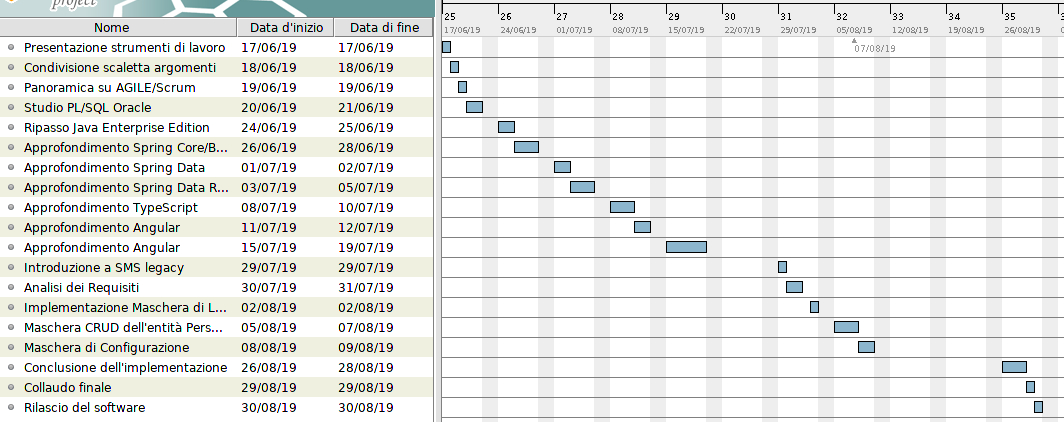
\includegraphics[width=1\columnwidth]{immagini/stage/gantt} 
	\caption{Diagramma di Gantt per la pianficazione dello stage}
	\label{figura:gantt-1}
\end{figure}

Sono presenti alcune settimane non aventi alcuna attività pianificata: ciò è dovuto a impegni pregressi pianificati dal sottoscritto e dalla chiusura dell'azienda per ferie.